\documentclass[]{exam}
\input{global}
\input{problem-sets}
\usepackage{circuitikz}
\ctikzset{bipoles/battery1/height=0.5}
\ctikzset{bipoles/battery1/width=0.25}
\ctikzset{bipoles/battery/height=0.4}
\ctikzset{bipoles/battery/width=0.2}
\ctikzset{bipoles/resistor/height=0.17}
\ctikzset{bipoles/resistor/width=0.38}
\ctikzset{bipoles/capacitor/width=0.1}
\ctikzset{bipoles/capacitor/height=0.4}
\ctikzset{bipoles/cuteswitch/thickness=0.3,bipoles/cuteswitch/shape=circ}
\ctikzset{bipoles/bulb/height=0.4,bipoles/bulb/width=0.4}
\usepackage{fontawesome}

\setrandomizerseed{1}
\bracketedpoints

\firstpageheader{{Name:\enspace\makebox[6cm]{\hrulefill}}\\{Physics}}{}{Test on Unit 11: Conservation of Charge}

% \newif\ifversionKlevel

% \versionKleveltrue

% \header{Physics \\Test on Unit 9: Conservation of Charge}{}{Name:\enspace\makebox[5cm]{\hrulefill}}

% \ifversionKlevel
%     \header{Physics \\Test on Unit 9: Conservation of Charge}{}{Name:\enspace\makebox[5cm]{\hrulefill}}
% \fi

\begin{document}

\subsection*{Electrostatics Quiz}

\begin{questions}
\question 
The SI unit of charge is the\ldots

\begin{randomizechoices}
    \choice Newton
    \correctchoice Ampere
    \choice Joule
    \choice Coulomb
\end{randomizechoices}

\question
Which of the charges shown in the image above is positive?

\begin{center}

\includegraphics[width=5cm]{documents/figures/electric-field-lines-6.pdf}
\end{center}

\begin{randomizechoices}[norandomize]
    \correctchoice A
    \choice B
    \choice Both A and B
    \choice Neither A nor B
\end{randomizechoices}

\question
Which statement best describes the image?

\begin{center}
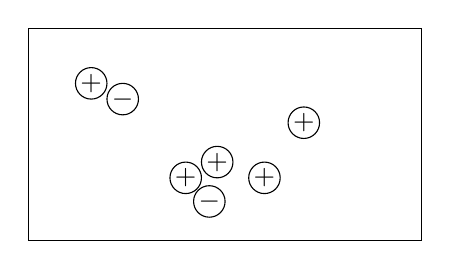
\begin{tikzpicture}
    \draw (0,0) rectangle (5,2.7);
    \draw (0.8,2) circle (0.2) node {$+$};
    \draw (1.2,1.8) circle (0.2) node {$-$};
    \draw (2,0.8) circle (0.2) node {$+$};
    \draw (2.4,1) circle (0.2) node {$+$};
    \draw (2.3,0.5) circle (0.2) node {$-$};
    \draw (3,0.8) circle (0.2) node {$+$};
    \draw (3.5,1.5) circle (0.2) node {$+$};
\end{tikzpicture}
\end{center}

\begin{randomizechoices}
    \correctchoice A positively charged object
    \choice A negatively charged object
    \choice A neutral object
    \choice There is not enough information to tell
\end{randomizechoices}

\question
According to Coulomb’s Law, if you increase the distance between two objects by a factor of 2, the electrical force between them will\ldots 

\begin{randomizechoices}
    \choice decrease by a factor of 2
    \choice increase by a factor of 2
    \correctchoice decrease by a factor of 4
    \choice increase by a factor of 4
\end{randomizechoices}

\question
(Needs fixing)
Which of the following velocity vectors represents the motion of the middle charge in the below diagram?

\question
A repelling force occurs between two charged objects when\ldots 

\begin{randomizechoices}
    \correctchoice charges are of like signs
    \choice charges are of equal magnitude
    \choice charges are of unlike signs
    \choice charges are of unequal magnitude
\end{randomizechoices}

\question
Which point charge in the image below has the strongest electric field?

\begin{center}
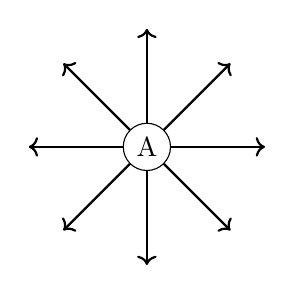
\begin{tikzpicture}[x=1.5cm,y=1.5cm]
    \foreach \x in {0,45,...,315}{
        \draw[->,thick,rotate=\x] (0,0) -- (1,0);
    }
    \draw[fill=white] (0,0) circle (3mm) node {A};
\end{tikzpicture}
\hspace{1cm}
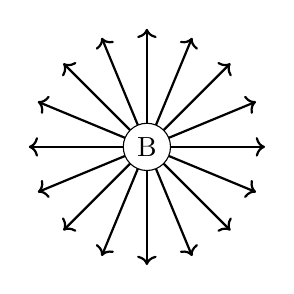
\begin{tikzpicture}[x=1.5cm,y=1.5cm]
    \foreach \x in {0,22.5,...,337.5}{
        \draw[->,thick,rotate=\x] (0,0) -- (1,0);
    }
    \draw[fill=white] (0,0) circle (3mm) node {B};
\end{tikzpicture}
\hspace{1cm}
\begin{tikzpicture}[x=1.5cm,y=1.5cm]
    {\ifprintanswers \color{red} \fi
    \foreach \x in {0,11.25,...,348.75}{
        \draw[->,thick,rotate=\x] (0,0) -- (1,0);
    }
    \draw[fill=white] (0,0) circle (3mm) node {C};
    }
\end{tikzpicture}
\end{center}

\begin{randomizechoices}[norandomize]
    \choice A
    \choice B
    \correctchoice C
    \choice Cannot determine
\end{randomizechoices}

\question
What particle(s) in the nucleus of an atom have an electric charge? (Select all that are correct.)

\begin{randomizechoices}[keeplast]
    \choice Electrons
    \correctchoice Protons
    \choice Neutrons
    \choice Megatrons
    \choice There are no particles in the nucleus
\end{randomizechoices}

\question
How does an object become negatively charged?

\begin{randomizechoices}
    \choice It loses protons.
    \correctchoice It gains electrons.
    \choice It gains neutrons.
    \choice It loses neutrons.
\end{randomizechoices}

\question
What is the difference between charging by conduction and charging by induction?

\begin{randomizechoices}
    \choice In conduction the objects don't touch, but in induction they do.
    \correctchoice In induction the objects don't touch, but in conduction they do.
    \choice Charges separate on the same side of one object in conduction.
    \choice Charges do not move in induction but they do in conduction.
\end{randomizechoices}

\question
While taking his clothes out of the dryer, Charles finds a sock clinging to his sweater. What is the best explanation for this common phenomenon? 

\begin{randomizechoices}[keeplast]
    \choice In the dryer, both the sock and the sweater lost electrons.
    \choice In the dryer, both the sock and the sweater gained electrons.
    \correctchoice In the dryer, either the sock or the sweater gained electrons while the other item lost electrons.
    \choice The cause of static cling is an unsolved scientific mystery.
\end{randomizechoices}

\question
Balloon A is known to have a positive charge.  Based on the experiments in the diagram below, determine the charge of Balloons B and C.

\begin{center}
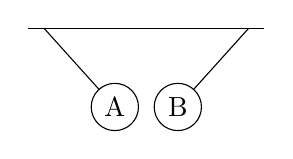
\begin{tikzpicture}
    \draw (0,0) -- (3,0);
    \draw (0.2,0) -- (1.1,-1);
    \draw (2.8,0) -- (1.9,-1);
    \draw[fill=white] (1.1,-1) circle (3mm) node {A};
    \draw[fill=white] (1.9,-1) circle (3mm) node {B};
\end{tikzpicture}
\hspace{1cm}
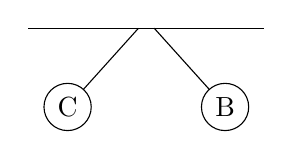
\begin{tikzpicture}
    \draw (0,0) -- (3,0);
    \draw (1.4,0) -- (0.5,-1);
    \draw (1.6,0) -- (2.5,-1);
    \draw[fill=white] (0.5,-1) circle (3mm) node {C};
    \draw[fill=white] (2.5,-1) circle (3mm) node {B};
\end{tikzpicture}
\end{center}

\begin{randomizechoices}
    \correctchoice Both B and C are negative.
    \choice B is positive and C is negative.
    \choice Both B and C are positive.
    \choice B is negative and C is positive.
\end{randomizechoices}

\question
Consider an isolated system consisting of two charges only. In the figure below, $Q_1$ is positive and $Q_2$ is negative.  How are the gravitational force and electrostatic force acting on $Q_1$ related to each other?

% \begin{center}
% \fbox{
\begin{minipage}{9cm}
\begin{randomizechoices}
    \correctchoice They are going in the same direction.
    \choice They are perpendicular.
    \choice The are going in opposite directions.
    \choice They are both 0.
\end{randomizechoices}
\end{minipage}
% }
%
% \fbox{
\begin{minipage}{3cm}
\centering
\begin{tikzpicture}
    \draw (0,2) -- (0,0) -- (2,0);
    \fill (0,1.5) circle (2pt) node[right=2pt] {$Q_1$};
    \fill (1.5,0) circle (2pt) node[below=2pt] {$Q_2$};
\end{tikzpicture}    
\end{minipage}
% }
% \end{center}

\question
Two particles with charges of $+4q$ and $-2q$ are a distance $3r$ apart. Which of the following is an expression for the magnitude of the electric force between them?
\smallskip

\begin{randomizeoneparchoices}
    \correctchoice $\displaystyle \frac{8kq^2}{9r^2}$
    \choice $\displaystyle \frac{8kq^2}{3r^2}$
    \choice $\displaystyle \frac{8kq^2}{r^2}$
    \choice $\displaystyle \frac{kq^2}{9r^2}$
\end{randomizeoneparchoices}

\question
A \SI{5}{\micro\coulomb} charge and a \SI{12}{\micro\coulomb} charge are located \SI{0.25}{m} apart. Calculate the electrostatic force acting between them.

\begin{solutionorbox}[4cm]
The electric force is given by Coulomb's law:

\begin{equation*}
    F = \frac{kq_1q_2}{r^2} = \frac{\left(\SI{9e9}{N\cdot m^2/C^2}\right)(\SI{5e-6}{C})(\SI{12e-6}{C})}{(\SI{0.25}{m})^2} = \boxed{\SI{8.64}{N}}
\end{equation*}
\end{solutionorbox}
\end{questions}

\clearpage

\subsection*{Circuits Quiz}

\begin{questions}
\question
Electrons are the mobile charge carriers in an electric circuit.

\begin{randomizechoices}[norandomize]
    \correctchoice True
    \choice False
\end{randomizechoices}

\question
Which of the following components are present in this diagram?

\begin{center}
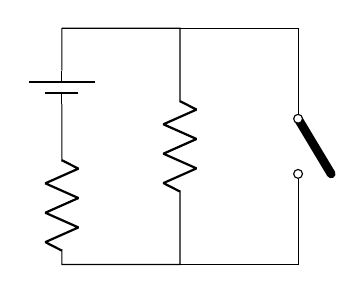
\begin{tikzpicture}[x=1.5cm,y=1.5cm]
    \draw (0,2) to[battery1] (0,1) to[R] (0,0) -- (1,0) to[R] (1,2) -- (0,2);
    \draw (1,2) -- (2,2) to[cute open switch] (2,0) -- (1,0);
\end{tikzpicture}
\end{center}

\begin{randomizechoices}
    \choice Bulb, switch, battery
    \choice Variable resistor, diode, battery
    \correctchoice Switch, resistors, battery
    \choice Resistor, switch, capacitor
\end{randomizechoices}

\question
Which of the following household devices uses the most power when plugged into a \SI{120}{V} outlet?

\begin{randomizechoices}[keeplast]
    \choice A laptop at \SI{1.0}{A}.
    \choice A video game player and TV that use \SI{3.2}{A} total.
    \correctchoice A microwave oven at \SI{4.2}{A}.
    \choice A cell phone charger that uses \SI{0.1}{A}.
    \choice All devices above run at the same power.
\end{randomizechoices}

\question
The flow of electricity requires a\ldots 

\begin{randomizechoices}
    \correctchoice complete path
    \choice complex circuit
    \choice insulated current
    \choice incomplete path
\end{randomizechoices}

\question
If a light bulb has a current of \SI{4.5}{A} and a resistance of \SI{3.2}{\ohm}, what is the voltage across the bulb?

\begin{randomizechoices}
    \choice \SI{0.7}{V}
    \choice \SI{1.4}{V}
    \correctchoice \SI{14.4}{V}
    \choice \SI{7.7}{V}
\end{randomizechoices}


\question
Identify the symbol shown in the image below.

\begin{center}
\begin{tikzpicture}
    \draw (1,0) to[battery1] (0,0);
\end{tikzpicture}
\end{center}

\begin{randomizechoices}
    \choice Wires
    \choice Switch
    \choice Light bulb
    \correctchoice Battery 
\end{randomizechoices}

\question
Which of the following refers to the electron flow in a circuit?

\begin{randomizechoices}
    \choice Power
    \choice Potential difference
    \choice Conductor
    \correctchoice Current
\end{randomizechoices}

\question
In this circuit, which branch has more current flowing through it?

\begin{center}
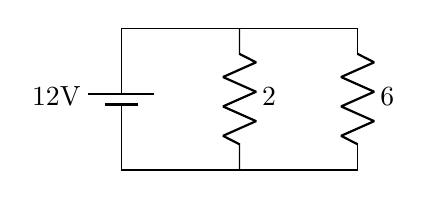
\begin{tikzpicture}[x=1.5cm,y=1.8cm]
    \draw (0,1) to[battery1,l_={\SI{12}{V}}] (0,0) -- (2,0) to[R,l_={\SI{6}{\ohm}}] (2,1) -- (0,1);
    \draw (1,1) to[R={\SI{2}{\ohm}}] (1,0);
\end{tikzpicture}
\end{center}

\begin{randomizechoices}[keeplast]
    \correctchoice The branch with the \SI{2}{\ohm} resistor.
    \choice The branch with the \SI{6}{\ohm} resistor.
    \choice Both branches have the same current.
    \choice There is not enough information to tell.
\end{randomizechoices}

\question
As the number of resistors increases in series across a battery, what happens to the voltage drop across each resistor?

\begin{randomizechoices}[keeplast]
    \correctchoice It decreases.
    \choice It stays the same.
    \choice It increases.
    \choice There is not enough information.
\end{randomizechoices}


\question
The electric current in a circuit will increase as the electric potential across a circuit is increased.

\begin{randomizechoices}[norandomize]
    \correctchoice True 
    \choice False
\end{randomizechoices}

\question
What is the current through a \SI{11}{V} bulb with a power of \SI{99}{W}?

\begin{randomizechoices}
    \choice \SI{60}{A}
    \choice \SI{99}{A}
    \correctchoice \SI{9.0}{A}
    \choice \SI{88}{A}
\end{randomizechoices}

\question
If the total resistance of the circuit shown is \SI{15}{\ohm}, what is the value of resistor $R$?

\begin{center}
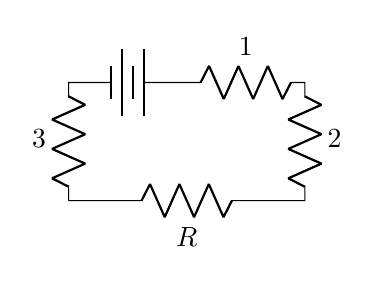
\begin{tikzpicture}[x=1.5cm,y=1.5cm]
    \draw (0,0) to[R,l_={$R$}] (2,0) to[R,l_={\SI{2}{\ohm}}] (2,1) to[R,l_={\SI{1}{\ohm}}] (1,1) to[battery] (0,1) to[R,l_={\SI{3}{\ohm}}] (0,0);
\end{tikzpicture}
\end{center}

\begin{randomizechoices}
    \correctchoice \SI{9}{\ohm}
    \choice \SI{12}{\ohm}
    \choice \SI{18}{\ohm}
    \choice \SI{6}{\ohm}
\end{randomizechoices}

\begin{solution}
In series, the total resistance is given by

\begin{equation*}
    R_\mathrm{eq} = R_1 + R_2 + R_3 + R
\end{equation*}

We know that $R_\mathrm{eq} = \SI{15}{\ohm}$. So,

\begin{equation*}
    \SI{15}{\ohm} = \SI{1}{\ohm} + \SI{2}{\ohm} + \SI{3}{\ohm} + R
\end{equation*}

which simplifies to

\begin{equation*}
    \SI{15}{\ohm} = \SI{6}{\ohm} + R
\end{equation*}

Therefore, solving for $R$, we get

\begin{equation*}
    R = \SI{15}{\ohm} - \SI{6}{\ohm} = \boxed{\SI{9}{\ohm}}
\end{equation*}
\end{solution}

\question
What is the power of a \SI{10}{V} bulb with \SI{5}{A} through it?

\begin{randomizechoices}
    \choice \SI{2}{V}
    \choice \SI{2}{W}
    \choice \SI{50}{A}
    \correctchoice \SI{50}{W}
\end{randomizechoices}


\begin{solution}
Power is

\begin{equation*}
    P = IV = (\SI{5}{A})(\SI{10}{V}) = \boxed{\SI{50}{W}} 
\end{equation*}
\end{solution}

\question
What is the total resistance of the circuit?

\begin{center}
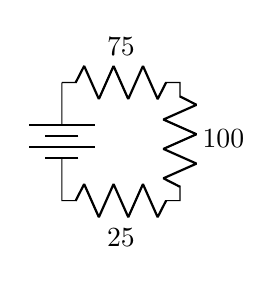
\begin{tikzpicture}[x=1.5cm,y=1.5cm]
    \draw (0,1) to[battery] (0,0) to[R,l_={\SI{25}{\ohm}}] (1,0) to[R,l_={\SI{100}{\ohm}}] (1,1) to[R,l_={\SI{75}{\ohm}}] (0,1);
\end{tikzpicture}
\end{center}

\begin{randomizechoices}
    \choice \SI{15.8}{\ohm}
    \correctchoice \SI{200}{\ohm}
    \choice \SI{0.63}{\ohm}
    \choice \SI{100}{\ohm}
\end{randomizechoices}

\begin{solution}
In series, total resistance is the sum of resistances:

\begin{align*}
    R_\mathrm{eq} &= R_1 + R_2 + R_3 \\[1ex]
    &= \SI{75}{\ohm} + \SI{100}{\ohm} + \SI{25}{\ohm} \\[1ex]
    &= \boxed{\SI{200}{\ohm}}
\end{align*}
\end{solution}

\question
The diagram below represents part of an electric circuit containing three parallel resistors.

\begin{center}
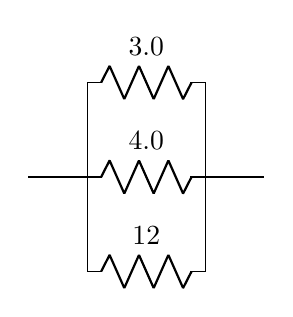
\begin{tikzpicture}[x=1.5cm,y=1.2cm]
    \draw (0,0) to[R={\SI{12}{\ohm}}] (1,0) -- (1,2) to[R,l_={\SI{3.0}{\ohm}}] (0,2) -- (0,0);
    \draw[shift={(-0.5,1)}] (0,0) to[R={\SI{4.0}{\ohm}}] (2,0);
\end{tikzpicture}
\end{center}


What is the equivalent resistance of this part of the circuit?

\begin{randomizechoices}
    \choice \SI{6.3}{ohms}
    \correctchoice \SI{1.5}{ohms}
    \choice \SI{0.67}{ohms}
    \choice \SI{19}{ohms}
\end{randomizechoices}

\begin{solution}
\begin{align*}
    R_\mathrm{eq} &= \left(\frac{1}{R_1} + \frac{1}{R_2} + \frac{1}{R_3}\right)^{-1} \\[1ex]
    &= \left(\frac{1}{\SI{3.0}{\ohm}} + \frac{1}{\SI{4.0}{\ohm}} + \frac{1}{\SI{12}{\ohm}}\right)^{-1} \\[1ex]
    &= \boxed{\SI{1.5}{\ohm}}
\end{align*}
\end{solution}
\end{questions}

\clearpage

\subsection*{Test on Unit 11}

\begin{questions}

% \question
% All wires shown below are made of the same material. Which wires shown has the smallest resistance?

% \begin{center}
% \begin{tikzpicture}
% \node[cylinder, 
% 	draw,
%         % text={black!5},
% 	cylinder uses custom fill, 
% 	cylinder body fill = black!5, 
% 	cylinder end fill = black!20,
% 	minimum height = 2cm,
%         minimum width=1cm] (c) at (0,0) {Wire 1};
%     \node[xshift=-1pt] at (1,0) {$A$};
%     \draw[|<->|,shift={(0,0.8)}] (-0.8,0) -- (1,0) node[above,pos=0.5] {$L$};
% \end{tikzpicture}
% \hspace{1cm}
% \begin{tikzpicture}
% \node[cylinder, 
% 	draw,
%         % text={black!5},
% 	cylinder uses custom fill, 
% 	cylinder body fill = black!5, 
% 	cylinder end fill = black!20,
% 	minimum height = 2cm,
%         minimum width=1.5cm] (c) at (0,0) {Wire 2};
%     \draw[rounded corners=2mm] (0.9,0) -- (1.3,0.1) -- (1.6,0.25) node[right] {$2A$};
%     \draw[|<->|,shift={(0,1)}] (-0.8,0) -- (1,0) node[above,pos=0.5] {$L$};
% \end{tikzpicture}
% \hspace{1cm}
% \begin{tikzpicture}
% \node[cylinder, 
% 	draw,
%         % text={black!5},
% 	cylinder uses custom fill, 
% 	cylinder body fill = black!5, 
% 	cylinder end fill = black!20,
% 	minimum height = 4cm,
%         minimum width=1cm] (c) at (0,0) {Wire 3};
%     \node at (1.9,0) {$A$};
%     \draw[|<->|,shift={(0,0.8)}] (-1.7,0) -- (1.9,0) node[above,pos=0.5] {$2L$};
% \end{tikzpicture}
% \end{center}

% \medskip

% \begin{randomizechoices}[norandomize]
%     \choice Wire 1
%     \correctchoice Wire 2
%     \choice Wire 3
%     \choice There is not enough information to tell. 
% \end{randomizechoices}


% \begin{solution}
% Resistance is proportional to length and inversely proportional to surface area:

% \begin{equation*}
%     R \propto \frac{L}{A}
% \end{equation*}

% Therefore, the wire with the least length and greatest area will have the smallest resistance: Wire 2.
% \end{solution}

\question
A positively charged rod touches a neutral metal sphere. The rod becomes less positive and the metal sphere now has an excess of positive charge. The redistribution of charge happens because \fillin[electrons] move from the sphere to the rod.

\begin{randomizechoices}
    \choice Neutrons
    \correctchoice Electrons
    \choice Atoms
    \choice Protons
\end{randomizechoices}

\question
Which of the charges shown in the image below is negative?

\begin{center}
    
\includegraphics[width=6cm]{documents/figures/electric-field-lines-1.pdf}
\end{center}

\begin{randomizechoices}[norandomize]
    \choice A
    \correctchoice B
    \choice Both
    \choice Neither
\end{randomizechoices}

\question
According to Coulomb’s Law, if the charge on two objects increases, how will the electrical force between them change?

\begin{randomizechoices}
    \choice The electrical force will stay the same.
    \correctchoice The electrical force will increase.
    \choice The electrical force will decrease.
    \choice There is not enough information to determine the effect.
\end{randomizechoices}

\question
As clothes in the dryer tumble and rub back and forth, electrons are scrubbed from one object to another. Why do the clothes stick together?

\begin{randomizechoices}
    \choice The friction between the clothes binds them together.
    \choice The electrons form a bond that is shared between the clothes.
    \correctchoice There is an overall positive charge on one item of clothes that loses electrons and it is attracted to the piece that has an overall negative charge from gaining electrons.
    \choice The weak nuclear force holds these items together.
\end{randomizechoices}

\question
In the diagram below, a negatively charged rod is placed between but does not touch identical small metal spheres R and S hanging from insulating threads. 

\begin{center}


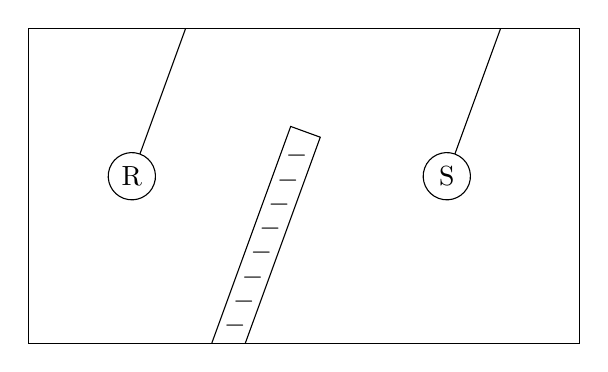
\begin{tikzpicture}[x=2cm,y=2cm]
    \begin{scope}
    \clip (-2,0) rectangle (1.5,-2);    
        \begin{scope}[rotate around={-20:(-1,0)}]
            \draw (-1,0) -- (-1,-1);
            \draw[fill=white] (-1,-1) circle (0.15) node {R};
        \end{scope}
        \begin{scope}[rotate around={-20:(+1,0)}]
            \draw (+1,0) -- (1,-1);
            \draw[fill=white] (1,-1) circle (0.15) node {S};
        \end{scope}
    
        \def\L{1.8}        % rod length
        \def\n{10}       % number of charges
        \def\top{-0.7} % top of rod
    
        \begin{scope}[rotate around={-20:(0,0)}]
            % rod
            \draw (-0.1,\top) rectangle ++(0.2,-\L);
    
            % evenly spaced charges
            \foreach \i in {1,...,\n}
            {
                \node at (0,{\top - \i*\L/(\n+1)}) {$-$};
            }
        \end{scope}
    \end{scope}
    \draw (-2,0) rectangle (1.5,-2);
\end{tikzpicture}
\end{center}

Which of the following statements regarding the spheres and rod are true in this situation? Select TWO correct answers.

\begin{randomizechoices}
    \choice Sphere R is positive or neutral.
    \choice Sphere S is positive or neutral
    \choice Sphere R is negative or neutral.
    \choice Sphere S is negative or neutral.
    \choice Sphere R must be negative.
    \choice Sphere S must be negative
\end{randomizechoices}


\question
What is the force between two charged spheres, each having a charge of $+\SI{2}{C}$, which are a distance of \SI{3}{m} apart?

\begin{randomizechoices}
    \choice \SI{9e9}{N}
    \choice \SI{4e9}{N}
    \correctchoice \SI{12e9}{N}
    \choice \SI{2e9}{N}
\end{randomizechoices}

\question
Two point charges, initially \SI{1}{cm} apart, are moved to a distance of \SI{3}{cm} apart. By what factor do the resulting electric and gravitational forces between them change?

\begin{randomizechoices}
    \choice The forces decrease by $1/3$.
    \correctchoice The forces decrease by $1/9$
    \choice The forces increase by $3$.
    \choice The forces increase by $9$
\end{randomizechoices}

\question
Electric fields point

\begin{randomizechoices}
    \correctchoice away from positive charge and towards negative charge
    \choice away from negative charge and towards positive charge
    \choice from left to right
    \choice away from the big charge and towards the little charge  
\end{randomizechoices}

\question
The diagram below shows two identical metal spheres, 1 and 2, separated by distance $d$. Each sphere has mass $m$ and possesses the charges shown below. The system consists of the two charges \underline{only}; the system does \textit{not} include the Earth.

\begin{center}
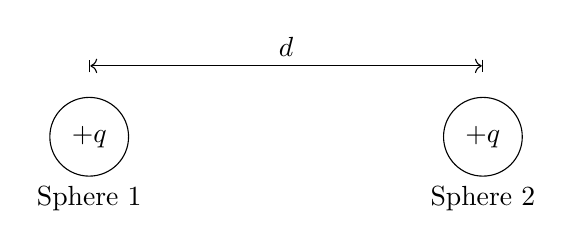
\begin{tikzpicture}
    \draw (0,0) circle (5mm) node {$+q$} node[below=5mm] {Sphere 1};
    \draw (5,0) circle (5mm) node {$+q$} node[below=5mm] {Sphere 2};
    \draw[|<->|,shift={(0,0.9)}] (0,0) -- (5,0) node[pos=0.5,above] {$d$};
\end{tikzpicture}
\end{center}

Which diagram best represents the electrostatic force $F_e$ and the gravitational force $F_g$ acting on Sphere~2 due to Sphere 1?

\begin{center}
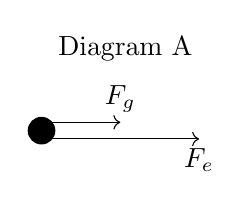
\begin{tikzpicture}
    \fill (0,0) circle (5pt);
    \draw[yshift=+3pt,->] (0,0) -- (1,0) node[above] {$F_g$};
    \draw[yshift=-3pt,->] (0,0) -- (2,0) node[below] {$F_e$};
    \node[above=2pt] at (current bounding box.north) {Diagram A};
\end{tikzpicture}
\hspace{7mm}
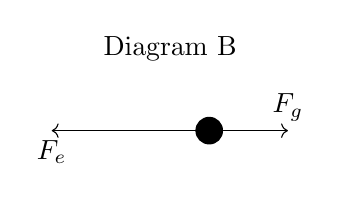
\begin{tikzpicture}
    \draw[yshift=+3pt,->,white] (0,0) -- (1,0) node[above] {$F_g$}; %...FOR ALIGNMENT ONLY
    \draw[yshift=-3pt,->,white] (0,0) -- (1,0) node[below] {$F_e$}; %...FOR ALIGNMENT ONLY
    \fill (0,0) circle (5pt);
    \draw[->] (0,0) -- (1,0) node[above] {$F_g$};
    \draw[->] (0,0) -- (-2,0) node[below] {$F_e$};
    \node[above=2pt] at (current bounding box.north) {Diagram B};
\end{tikzpicture}
\hspace{7mm}
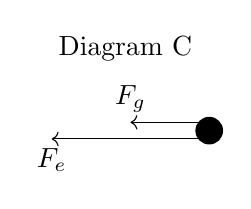
\begin{tikzpicture}
    \fill (0,0) circle (5pt);
    \draw[yshift=+3pt,->] (0,0) -- (-1,0) node[above] {$F_g$};
    \draw[yshift=-3pt,->] (0,0) -- (-2,0) node[below] {$F_e$};
    \node[above=2pt] at (current bounding box.north) {Diagram C};
\end{tikzpicture}
\hspace{7mm}
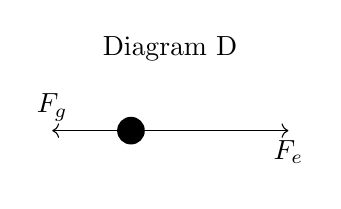
\begin{tikzpicture}
    \draw[yshift=+3pt,->,white] (0,0) -- (1,0) node[above] {$F_g$}; %...FOR ALIGNMENT ONLY
    \draw[yshift=-3pt,->,white] (0,0) -- (1,0) node[below] {$F_e$}; %...FOR ALIGNMENT ONLY
    \fill (0,0) circle (5pt);
    \draw[->] (0,0) -- (-1,0) node[above] {$F_g$};
    \draw[->] (0,0) -- (+2,0) node[below] {$F_e$};
    \node[above=2pt] at (current bounding box.north) {Diagram D};
\end{tikzpicture}
\end{center}

\begin{randomizeoneparchoices}[norandomize]
    \choice Diagram A
    \choice Diagram B
    \choice Diagram C
    \correctchoice Diagram D
\end{randomizeoneparchoices}

\question
The magnitude of the electrostatic force between two charged particles is directly proportional to the product of the magnitude of the charges and inversely proportional to the square of the distance between them. This statement best describes

\begin{randomizechoices}
    \correctchoice Coulomb's Law
    \choice Coulomb's Constant
    \choice Newton's 3rd Law
    \choice Newton's 2nd Law
    \choice Newton's 1st Law 
\end{randomizechoices}

\question
Which of the following labeled points is in the region with the greatest magnitude of electric field?

\begin{center}
    
\includegraphics[width=6cm]{documents/figures/electric-field-lines-2.pdf}
\end{center}

\begin{randomizeoneparchoices}[norandomize]
    \choice Point A
    \correctchoice Point B
    \choice Point C
    \choice Point D
    \choice Point E
\end{randomizeoneparchoices}

\question
Which diagram shows a series circuit?

\begin{center}
\begin{minipage}{4.4cm}
\centering
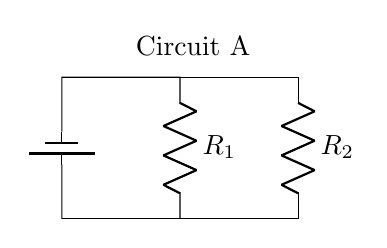
\begin{tikzpicture}[x=1.5cm,y=1.8cm]
    \draw (0,0) to[battery1] (0,1) -- (1,1) to[R={$R_1$}] (1,0);
    \draw (1,1) -- (2,1) to[R={$R_2$}] (2,0) -- (0,0); 
    \node[above=4pt] at (current bounding box.north) {Circuit A};
\end{tikzpicture}
\end{minipage}%
\begin{minipage}{3.4cm}
\centering
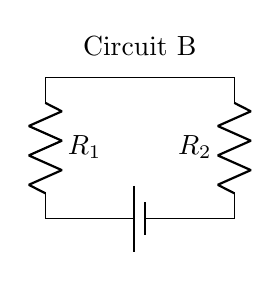
\begin{tikzpicture}[x=1.2cm,y=1.8cm]
    \draw (0,0) to[battery1] (2,0) to[R={$R_2$}] (2,1) -- (0,1) to[R={$R_1$}] (0,0);
    \node[above=4pt] at (current bounding box.north) {Circuit B};
\end{tikzpicture}
\end{minipage}%
\begin{minipage}{3.5cm}
\centering
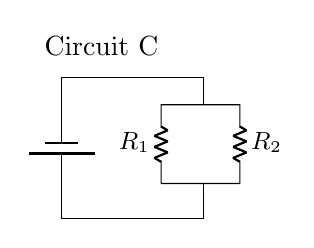
\begin{tikzpicture}[x=1.8cm,y=1.8cm]
    \draw (0,0) to[battery1] (0,1) -- (1,1) -- (1,0) -- (0,0);
    \begin{scope}[shift={(0.7,0.25)},x=1cm,y=1cm]
        \small
        \ctikzset{bipoles/resistor/height=0.12}
        \ctikzset{bipoles/resistor/width=0.3}
        \fill[white] (0,0) rectangle (1,1);
        \draw (0,0) to[R={$R_1$}] (0,1) -- (1,1) to[R={$R_2$}] (1,0) -- (0,0);
    \end{scope}
    \node[above=4pt,xshift=-2em] at (current bounding box.north) {Circuit C};
\end{tikzpicture}
\end{minipage}%
\begin{minipage}{3cm}
\centering
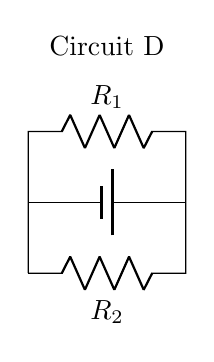
\begin{tikzpicture}[x=1cm,y=1.8cm]
    \draw (0,0) to[R,l_={$R_2$}] (2,0) -- (2,1) to[R,l_={$R_1$}] (0,1) -- (0,0);
    \draw (2,0.5) to[battery1] (0,0.5);
    \node[above=4pt] at (current bounding box.north) {Circuit D};
\end{tikzpicture}
\end{minipage}
\end{center}

\scalebox{0}{
\begin{randomizeoneparchoices}[norandomize]
    \choice Circuit A
    \correctchoice Circuit B
    \choice Circuit C
    \choice Circuit D
\end{randomizeoneparchoices}
}

\question
A circuit is set up as show below.  What is wrong with the figure?

\begin{center}
\begin{tikzpicture}[x=3cm,y=1.5cm]
    \draw (0,0) to[battery1] (0,1) -- (1,1) -- (1,0);
    \draw (0,0) to[cute open switch] (1,0);
    \begin{scope}[shift={(0.5,1.1)}]
        \foreach \x in {20,40,...,160}{
            \draw[thick,rotate=\x] (0,0) -- (0.3,0);
        }
        \fill[white] (0,0.11) circle (3.5mm);
        \node at (0,0) {\resizebox{5mm}{!}{\faLightbulbO}};
    \end{scope}
\end{tikzpicture}
\end{center}

\begin{randomizechoices}[keeplast]
    \correctchoice The switch is open but the light bulb is on.
    \choice  The light bulb will short the circuit.
    \choice No power supply is shown.
    \choice Nothing is wrong with the image.
\end{randomizechoices}

\question
A light bulb has a resistance of \SI{1.2}{\ohm}. What is the voltage across the light bulb when a current of \SI{4}{A} flows through it?

\begin{randomizeoneparchoices}
    \correctchoice \SI{4.8}{V}
    \choice \SI{0.3}{V}
    \choice \SI{3.3}{V}
    \choice \SI{5.2}{V}
\end{randomizeoneparchoices}

\clearpage

\question
Initially, a \SI{75}{W} light bulb operates at a voltage of \SI{120}{V}. If the bulb wattage was doubled, what would happen to current through the battery?

\begin{randomizechoices}[keeplast]
    \correctchoice The current would double.
    \choice The current would stay the same.
    \choice The current would be halved.
    \choice There is not enough information to tell.
\end{randomizechoices}

\begin{solution}
The power dissipated by a circuit element is

\begin{equation*}
    P=IV
\end{equation*}

Therefore, doubling the power while keeping voltage constant requires that the current through the element be doubled too.
\end{solution}

\question
What kind of circuit is shown below?

\begin{center}
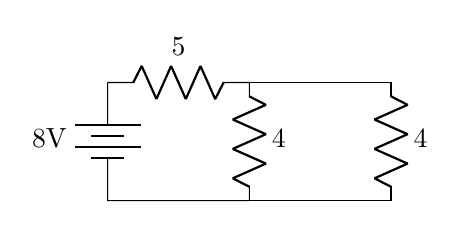
\begin{tikzpicture}[x=1.8cm,y=1.5cm]
    \draw (0,1) to[battery,l_={\SI{8}{V}}] (0,0) -- (1,0) to[R,l_={\SI{4}{\ohm}}] (1,1) to[R,l_={\SI{5}{\ohm}}] (0,1);
    \draw (1,0) -- (2,0) to[R,l_={\SI{4}{\ohm}}] (2,1) -- (1,1);
\end{tikzpicture}
\end{center}

\begin{randomizeoneparchoices}
    \choice Short circuit
    \choice Series circuit
    \correctchoice Combination circuit
    \choice Parallel circuit
\end{randomizeoneparchoices}

\question
Your house is wired in

\begin{randomizechoices}
    \choice parallel, so that if something is unplugged everything else goes off.
    \choice series, so that if something is unplugged everything else goes off.
    \correctchoice parallel, so that if something is unplugged everything else is fine.
    \choice series, so that is something is unplugged everything else is fine.
\end{randomizechoices}

\question
A 125 volt battery delivers a current of 2.0 amperes to a portable radio. If the resistance in the circuit was doubled, what would happen to the current?

\begin{randomizechoices}[keeplast]
    \choice The current would remain the same.
    \correctchoice There current would be cut in half.
    \choice The current would double.
    \choice There is not enough information to tell.
\end{randomizechoices}

\begin{solution}
Ohm's law states

\begin{equation*}
    I = \frac{V}{R}
\end{equation*}

Therefore, if resistance is doubled while voltage remains constant, the current must decrease by one-half.
\end{solution}

\question
Three resistors, \SI{4}{\ohm}, \SI{6}{\ohm}, and \SI{8}{\ohm}, are connected in parallel in an electric circuit. The equivalent resistance $R_\mathrm{eq}$ of the circuit is
\bigskip

\begin{randomizeoneparchoices}
    \choice $\SI{4}{\ohm} < R_\mathrm{eq} < \SI{8}{\ohm}$
    \choice $R_\mathrm{eq} = \SI{18}{\ohm}$
    \correctchoice $R_\mathrm{eq} < \SI{4}{\ohm}$
    \choice $\SI{10}{\ohm} < R_\mathrm{eq} < \SI{19}{\ohm}$
\end{randomizeoneparchoices}

% \begin{randomizechoices}
%     \choice Between \SI{4}{\ohm} and \SI{8}{\ohm} 
%     \choice \SI{18}{\ohm}
%     \choice Between \SI{10}{\ohm} and \SI{19}{\ohm}
%     \correctchoice Less than \SI{4}{\ohm}
% \end{randomizechoices}

\question
Which combination of resistors has the smallest equivalent resistance?

\begin{center}
\begin{minipage}{3.8cm}
\centering
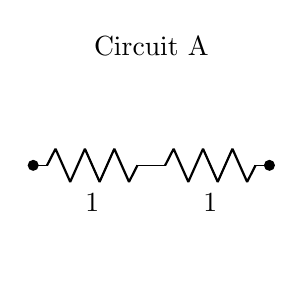
\begin{tikzpicture}[x=1.5cm]
    \draw (0,0) to[R,l_={\SI{1}{\ohm}}] (1,0) to[R,l_={\SI{1}{\ohm}}] (2,0);
    \fill (0,0) circle (2pt);
    \fill (2,0) circle (2pt);
    \phantom{%...for alignment only
        \begin{scope}[shift={(0.5,-0.5)}]
            \fill[white] (0,0) rectangle (1,1);
            \draw (0,0) -- (0,1) to[R={\SI{0}{\ohm}}] (1,1) -- (1,0) to[R={\SI{0}{\ohm}}]  (0,0);
        \end{scope}
    }
    \node[above=2pt] at (current bounding box.north) {Circuit A};
\end{tikzpicture}
\end{minipage}%
\begin{minipage}{3.8cm}
\centering
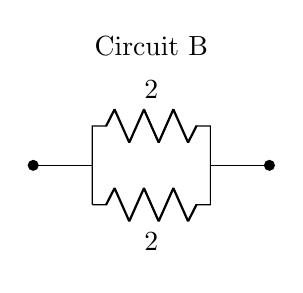
\begin{tikzpicture}[x=1.5cm]
    \draw (0,0) -- (2,0);
    \begin{scope}[shift={(0.5,-0.5)}]
        \fill[white] (0,0) rectangle (1,1);
        \draw (0,0) -- (0,1) to[R={\SI{2}{\ohm}}] (1,1) -- (1,0) to[R={\SI{2}{\ohm}}]  (0,0);
    \end{scope}
    \fill (0,0) circle (2pt);
    \fill (2,0) circle (2pt);
    \node[above=2pt] at (current bounding box.north) {Circuit B};
\end{tikzpicture}
\end{minipage}
\begin{minipage}{3.8cm}
\centering
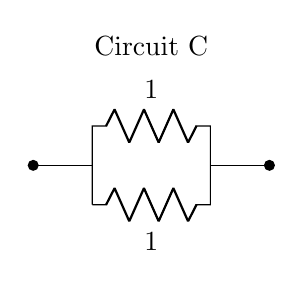
\begin{tikzpicture}[x=1.5cm]
    \draw (0,0) -- (2,0);
    \begin{scope}[shift={(0.5,-0.5)}]
        \fill[white] (0,0) rectangle (1,1);
        \draw (0,0) -- (0,1) to[R={\SI{1}{\ohm}}] (1,1) -- (1,0) to[R={\SI{1}{\ohm}}]  (0,0);
    \end{scope}
    \fill (0,0) circle (2pt);
    \fill (2,0) circle (2pt);
    \node[above=2pt] at (current bounding box.north) {Circuit C};
\end{tikzpicture}
\end{minipage}
\begin{minipage}{3.8cm}
\centering
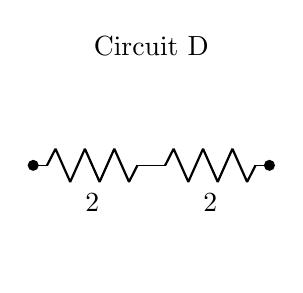
\begin{tikzpicture}[x=1.5cm]
    \draw (0,0) to[R,l_={\SI{2}{\ohm}}] (1,0) to[R,l_={\SI{2}{\ohm}}] (2,0);
    \fill (0,0) circle (2pt);
    \fill (2,0) circle (2pt);
    \phantom{%...for alignment only
        \begin{scope}[shift={(0.5,-0.5)}]
            \fill[white] (0,0) rectangle (1,1);
            \draw (0,0) -- (0,1) to[R={\SI{0}{\ohm}}] (1,1) -- (1,0) to[R={\SI{0}{\ohm}}]  (0,0);
        \end{scope}
    }
    \node[above=2pt] at (current bounding box.north) {Circuit D};
\end{tikzpicture}
\end{minipage}
\end{center}

\scalebox{0}{
\begin{randomizeoneparchoices}[norandomize]
    \choice Circuit A
    \choice Circuit B
    \correctchoice Circuit C
    \choice Circuit D
\end{randomizeoneparchoices}
}

\begin{solution}
The equivalent resistance in the parallel Circuit C is

\begin{equation*}
    R_\mathrm{eq} = \left(\frac{1}{\SI{1}{\ohm}} + \frac{1}{\SI{1}{\ohm}}\right)^{-1} = \SI{0.5}{\ohm}
\end{equation*}

All other circuits have bigger equivalent resistances.
\end{solution}

\question
In the diagram below, if the circuit breaks at Point 1, which light bulb(s) remain on?

\begin{center}
\begin{tikzpicture}[y=1.8cm]
    \draw (0,0) to[battery] (0,1) -- (3,1) -- (3,0) -- (0,0);
    \draw (1,1) -- (1,0);
    \draw (2,1) -- (2,0);
    \draw (1,0.4) node[fill=white] {\faLightbulbO} node[above left=2pt] {X};
    \draw (2,0.4) node[fill=white] {\faLightbulbO} node[above left=2pt] {Y};
    \draw (3,0.4) node[fill=white] {\faLightbulbO} node[above left=2pt] {Z};
    \fill (2,0.8) circle (2pt);
    \draw[<-,thick,shift={(2pt,2pt)}] (2,0.8) -- ++(0.6,0.4) node[right] {Point 1};
\end{tikzpicture}
\end{center}

\begin{randomizeoneparchoices}
    \choice X and Y
    \correctchoice X and Z
    \choice Y and Z
    \choice None of them
\end{randomizeoneparchoices}









\end{questions}


\end{document}